%%%%%%%%%%%%%%%%%%%%%%%%%%%%%%%%%%%%%%%%%%%%%%%%%%%%%%%%%%%%%%%%%%%%%%%%
%                                                                      %
%     File: Horizon_extension.tex                                      %
%     Tex Master: Thesis.tex                                           %
%                                                                      %
%     Author: Israel Sother                                            %
%     Last modified: 27 May 2024                                       %
%                                                                      %
%%%%%%%%%%%%%%%%%%%%%%%%%%%%%%%%%%%%%%%%%%%%%%%%%%%%%%%%%%%%%%%%%%%%%%%%
\subsubsection{Horizon Extesion}
\label{section:Horizon Extesion}%chktex 24

A previously overlooked problem is the compensation of the computational time, as the acquisition and control calculations cannot be done instantly their delay needs to be compensated. The strategy adopted here is to use the motor model equations \Cref{eq:motor_backward_euler_matrix} coupled with the previously calculated control action to predict the system state in the next time step, this is called horizon extension. Usually, this is done in a fixed timestep manner, where the predictive controllers instead of picking the control action for $k$ in the timestep $k$, pick the control action for $k+1$ in the timestep $k$, as shown in \Cref{eq:horizon_default} where $x$ represent the currents, $u$ is the voltage vector, $A$, $B$, $C$, and $D$ are the matrices and vectors of the model in \Cref{eq:motor_backward_euler_matrix} and are all dependent on the prediction duration $h = \frac{1}{f_{sw}}$.
\begin{equation}
	x_{k+1} = A^{-1} \left (B x_k + C u_k + D\right )
	\label{eq:horizon_default}
\end{equation}

For this equation to work the system timeline needs to be as in \Cref{fig:horizon_default_timeline}, starting with taking the current and voltage measurements, followed by applying the voltage vectors calculated in $k-1$, then extending the horizon by one timestep, and calculating the voltage vector for the next timestep~\cite{Vazquez:MPC_uses:2014}.

\begin{figure}[!htb]
	\centering
	\includegraphics[width=1\textwidth]{Figures/Horizon Extension default Timeline.pdf}
	\caption[Horizon extension by one timestep.]{Horizon extension by one timestep.}
	\label{fig:horizon_default_timeline} %chktex 24
\end{figure}

This can be improved by only extending the horizon by the necessary time to compute the control action, this way the prediction error derived from model mismatch is reduced because the amount of time to predict is smaller. To do that the prediction duration is simply reduced to $h = t_{control}$, while the system timeline is shifted as in \Cref{fig:horizon_extend_timeline}. The combination of explicitly solving the \gls{mpc} model equation with the hybrid horizon timestep approach, where the horizon extension has a shorter timestep than the controllable horizon is called \acrfull{rush}. It has the benefits of being a continuous set model predictive control, thus reducing the ripple, while being computationally efficient, as it is explicitly calculated, and reducing the prediction error due to model mismatch as it uses the reduced horizon extension technique.

\begin{figure}[!htb]
	\centering
	\includegraphics[width=1\textwidth]{Figures/Horizon Extension Timeline.pdf}
	\caption[Horizon Extension by control time.]{Horizon Extension by control time.}
	\label{fig:horizon_extend_timeline} %chktex 24
\end{figure}

The final control cycle starts with sensor acquisition, followed by horizon extension, and lastly the future control action computation. Note that this delay is not a problem with simulation in \textit{Simulink}, as it can instantly do the calculations, but it is good practice to simulate it with the proper delays to increase the similarity between simulation and experimental results.


\begin{figure}[!htb]
	\centering
	\begin{subfigmatrix}{2}
		\subfigure[Default Horizon Extention.]{
			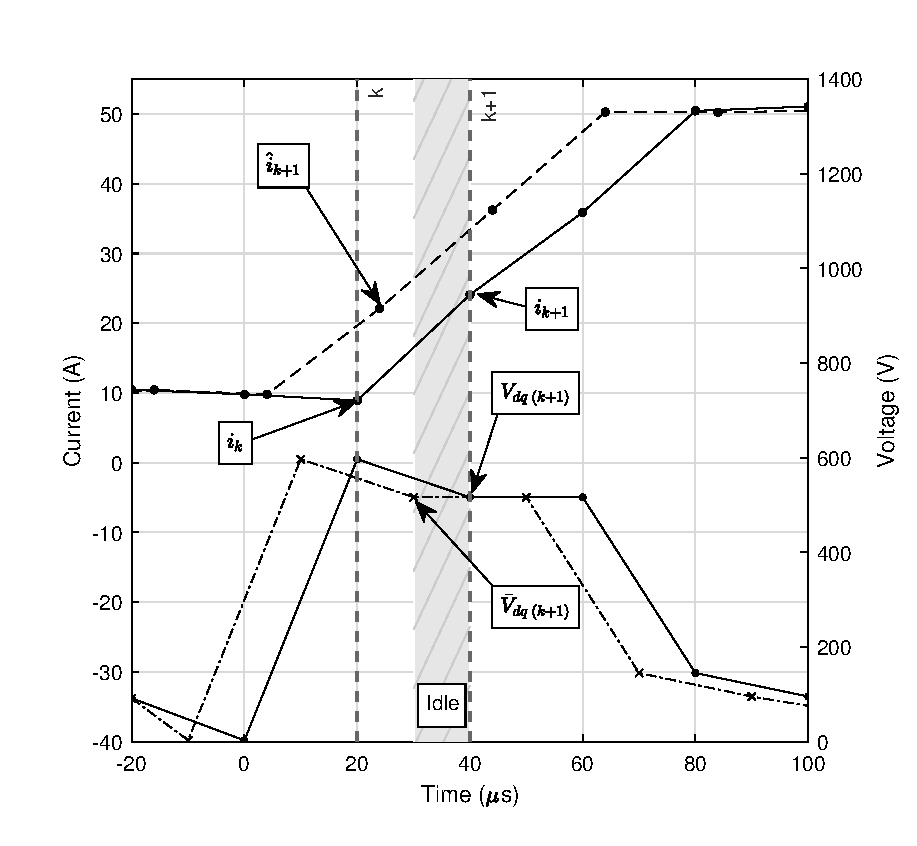
\includegraphics[width=.47\textwidth]{Figures/long_horizon.eps}
			\label{fig:normal_timeline}
		}
		\subfigure[Ultra Short Horizon Extention.]{
			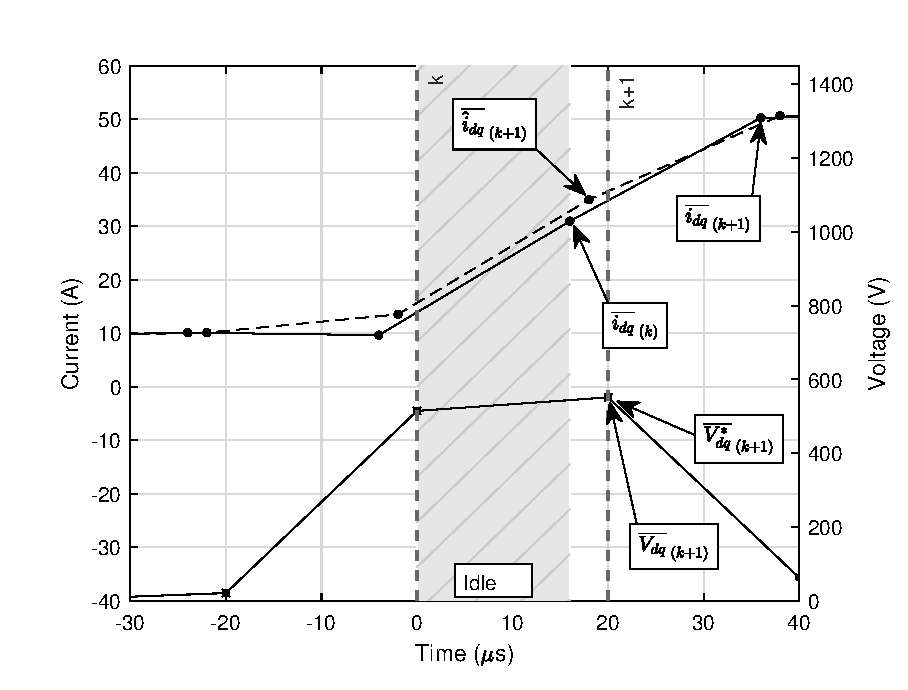
\includegraphics[width=.47\textwidth]{Figures/short_horizon.eps}
			\label{fig:USH_timeline}
		}
	\end{subfigmatrix}
	\caption{Horizon extension comparison, on top the measured and predicted voltages. The bottom lines are the computed control action and the applied control action}
	\label{fig:hor_comparison}
\end{figure}

A comparison of the diferente horizon extension methods is shown in \Cref{fig:hor_comparison}. The lines on the top represent the predicted and measured currents, while the lower lines are the voltages. Note that the markers in this figure are placed on the exact time the hardware finishes each computation, thus the delay between measurement, extension, and control calculation. The dashed voltage line represents the control action at the computation time, so in the regular horizon extension it is ahead of the applied control action. The ultra short horizon technique allows it to be applied as soon as it is computed.
